% % \part{数学建模实战}
% % \chapter{超薄座椅}

% \documentclass[UTF8]{ctexbook}

% \ctexset{
%     part/number = \chinese{part}
% }

% \usepackage{multirow}
% \usepackage{amsmath}% ams 数学公式
% \usepackage{amsfonts}% ams 数学字体
% \usepackage{bbm}%重影字体
% \usepackage{amssymb,latexsym}% ams 数学符号与LaTeX数学符号
% \usepackage{mathrsfs}% 花式符号
% \usepackage{ntheorem}%定理、定义、证明
%     \theoremstyle{nonumberplain}
%     \theoremheaderfont{\bfseries}
%     \theorembodyfont{\normalfont}
%     \theoremsymbol{$\square$}
%     \newtheorem{Proof}{\hskip 2em 证明}
%     \newtheorem{theorem}{\hspace{2em}定理}[chapter]
%     \newtheorem{definition}{\hspace{2em}定义}[chapter] % 如果没有章, 只有节, 把上面的[chapter]改成[section]
%     \newtheorem{axiom}[definition]{\hspace{2em}公理}
%     \newtheorem{lemma}[definition]{\hspace{2em}引理}
%     \newtheorem{proposition}[definition]{\hspace{2em}命题}
%     \newtheorem{corollary}[definition]{\hspace{2em}推论}
%     \newtheorem{remark}{\hspace{2em}注}[chapter] %类似地定义其他“题头”. 这里“注”的编号与定义、定理等是分开的
%     \newtheorem{Assumption}{\hspace{2em}假设}[chapter]

% %算法伪代码
% %http://blog.csdn.net/lwb102063/article/details/53046265
% \usepackage{algorithm}
% \usepackage{algorithmicx}
% \usepackage{algpseudocode}
%     \floatname{algorithm}{算法}
%     \renewcommand{\algorithmicrequire}{\textbf{输入:}}
%     \renewcommand{\algorithmicensure}{\textbf{输出:}}
% % 罗马数字:示例:\rom{2}
% \makeatletter
% \newcommand*{\rom}[1]{\expandafter\@slowromancap\romannumeral #1@}
% \makeatother

% \usepackage{enumerate}%itemiz环境。\begin{enumerate}[step 1][a)]可以使用 A,a,I,i,1 作为可选项产生 \Alph,\alph,\Roman,\roman,\arabic 的效果
% \usepackage{cite}%参考文献
%     \bibliographystyle{plain}
% \usepackage{extarrows}% 带参数的箭头
% \usepackage{hyperref}% 超链接
% \usepackage{pifont}%然后在正文输入\ding{172}~\ding{211}得到相应数字,要是要①就输入:\ding{172}②就输:\ding{173}
% %\usepackage[CJKbookmarks, colorlinks, bookmarksnumbered=true,pdfstartview=FitH,linkcolor=black,citecolor=black]{hyperref}%超链接的格式设置
% \hypersetup{
%     colorlinks=false,% 去掉超链接颜色
%     pdfborder=0 0 0% 取消超链接的边框
% }
% \usepackage{graphicx}% 图片管理
% \usepackage{caption}
% \usepackage{subcaption}%并排的图各有标题
% \graphicspath{{images/}}% 设置图片搜索路径
% \usepackage{float,varwidth}% 浮动体
% \usepackage{booktabs}% 三线表
% \usepackage{fancyhdr}% 页眉设置
% \usepackage{xcolor}% 颜色宏包
% \usepackage{colortbl}% 彩色表格
% \usepackage{listings}% 代码高亮
% \usepackage{caption}% 对标题进行控制,如让\caption标题的字体缩小一号,同时数字标签使用粗体可以用:\usepackage[font=small,labelfont=bf]{caption}
% \usepackage{xfrac,upgreek}%分别是行间公式如a/b的形式(将原来的命令\frac改成\sfrac)和希腊字体的宏包的
% \usepackage{mathtools}%lgathered和rgathered环境把公式向左向右对齐
% \usepackage{tabularx}%提供自动延伸的表列,(X列格式说明符),文字过长时可以自动转行
% \usepackage{longtable}%长表格
% \usepackage{enumitem}%enumerate宏包的升级
% \usepackage{harpoon}%数学公式的矢量
% \usepackage{bookmark}%目录的书签
% \renewcommand{\headwidth}{\textwidth}%图片并排,这个要列在所有宏包的后面
% \definecolor{codegreen}{rgb}{0,0.6,0}
% \definecolor{codegray}{rgb}{0.5,0.5,0.5}
% \definecolor{codepurple}{rgb}{0.58,0,0.82}
% \definecolor{backcolour}{rgb}{0.95,0.95,0.92}
% \lstset{
%     commentstyle=\color{codegreen},
%     keywordstyle=\color{magenta},
%     numberstyle=\tiny\color{codegray},
%     stringstyle=\color{codepurple},
%     basicstyle=\footnotesize,
%     breakatwhitespace=false,% 断行只在空格处
%     breaklines=true,% 自动断行
%     captionpos=b,% 标题位置
%     keepspaces=true,
%     numbers=left,
%     numbersep=5pt,
%     showspaces=false,
%     showstringspaces=false,
%     showtabs=false,% 显示
%     tabsize=2% TAB 被当作两个空格
% }
% \topmargin=0pt\oddsidemargin=0pt\evensidemargin=0pt
% \textwidth=16.5cm\textheight=23cm\raggedbottom%我这么设置是为了缩小页边距,满足有的文字无法转行
% \pagestyle{headings}%页眉为章节标题,无页脚
% \setlength{\abovecaptionskip}{10pt}
% \setlength{\belowcaptionskip}{-15pt}%图片表格的前后距离设置
% \CTEXsetup[format={\zihao{-3}\raggedright\bfseries}]{section}%设置节的格式

% \begin{document}
% \part{数学建模实战}
\chapter{超薄座椅}
\section{题目要求}
    \par
    \textbf{Problem A(MCM): The slimline seats on the airplane}
    \par
    An airline seat is a seat on an airliner in which passengers are accommodated for the duration of the journey. Some airlines are now introducing new ”slimline” seats in economy class. These seats,in addition to weighing less, theoretically allow airlines to increase capacity without significantly affecting passenger comfort. These seats may or may not feature moveable headrests, and generally do not feature adjustable lumbar support. Slimline seats are being further refined, liberating more passenger space. The common point of them is a thinner backplate and less padding. However, many passengers have expressed displeasure with these seats.
    \par
    Without changing the structure of the premise, how to designseat back curve, in order to make the seat more comfortable?
    \par
    How to optimize the seat backplate curve and padding, in or-der to make the seat more comfortable, without changing the main internal structure? Please write an advertising material with 2-3 pages for the airline, to describe your design features and advantages concisely.

\section{超薄座椅的优化设计}
    \subsection{模型假设}
        \begin{enumerate}
        \item 假设人体背部曲线为以脊椎点为顶点的二次曲线;
        \item 假设人体背部侧面轮廓为直线;
        \item 只按照男性身高特征设计座椅。
        \end{enumerate}
    \subsection{符号说明}
    \subsection{问题一的分析与求解}
        \subsubsection{问题的分析}
            \par
            问题需要我们在保证不改变结构的前提下,设计座椅靠背曲线,以使所述座椅更加舒适。
            \par
            题目并没有给出飞机座椅的其它信息,因此,我们要自行查找材料。我们找到有关人体脊柱结构的数据,对这组数据进行插值与拟合,从中找出合理的脊柱曲线,并将脊柱曲线作为座椅的中轴线。
        \subsubsection{模型的建立与求解}
            \par
            \textbf{(1)脊柱模型}
            \par
            因为座椅设计的舒适度主要是靠人体脊椎感知的,为了设计舒适的座椅,我们筛选出人体脊椎的相关数据,即脊椎的主要结构(即尾骨、腰椎、胸椎、颈椎、后脑勺头肩宽,臀宽等)的相对距离(距离椅背的距离),如表(\ref{人体脊椎数据})所示。
            \begin{table}[H]
            \centering
            \caption{人体脊椎数据}
            \label{人体脊椎数据}
            \begin{tabular}{l|llllllllllllll}% 需要引入 tabularx 宏包;表格总宽度一定要设置
                \toprule
                % 命令 & 意义\\
                % \midrule
                $x_i$  &0 &  50 & 200& 240& 290& 330& 400& 500& 550& 610 & 670& 705&  790& 847\\
                $y_i$ &10&  0  & 7.3& $h_1$ & 10 & 7.9& 4.6& 1.5& 0  & 9.3 & $h_2$ & 7.3&  4  & 0\\
            \bottomrule
            \end{tabular}
            \end{table}
            \par
            这里值得注意的是,由于我们的脊椎数据并不是很完整(这个数据不容易查找),我们不得不想办法将其“填补”完整。查阅相关资料,我们发现人体脊椎曲线有一定的约束:合理的坐姿(脊椎曲线)在腰椎和肩胛骨这两个点的曲率分别为1000和500。在上面的数据中,我们并没有腰椎和肩胛骨这两点的数据,为此,我们将腰背凸起和头枕处凸起最高点到腰背直板处的距离记为$h_i$。
            其中:$h_1$,$h_2$分别表示腰靠和头枕处凸起的高度,且单位均为$mm$(即腰椎和肩胛骨距离椅背的距离)。
            \par
            下面的问题是:求解最优的$h_1,h_2$,使得人体脊椎曲线在腰椎和肩胛骨这两个点的曲率接近1000和500。思考一下,每给定一个$h_1,h_2$,我们就有一个脊椎曲线的离散点数据,我们可以根据这个数据来求解脊椎曲线$f$(插值或拟合),在求解出脊椎曲线$f$之后,我们就可以得到$f$在腰椎和肩胛骨这两个点的曲率$R_1,R_2$,最后,我们只要让$R_1,R_2$接近1000和500即可。
            \par
            设人体脊椎曲线为$f$,用$d(R_1,1000)$来衡量曲率$R_1$和1000之间的距离,我们可以设计模型
            \begin{align*}
            \min_{f\in \mathcal{F}} \ d(R_1,1000)+d(R_2,500)
            \end{align*}
            上述问题是一个泛函问题,并且由于不存在约束,必然存在最优的$f^*\in F$,使得目标最小。下面我们来考虑添加约束,设脊椎曲线的测量点为$(x_i,y_i)$,(1)我们可以要求测量点就在脊椎曲线$f$上,换句话说,$f$必过$x_i,y_i$,于是我们可以设计模型
            \begin{align*}
            & \min_{f\in \mathcal{F}} \ d(R_1,1000)+d(R_2,500)\\
            & s.t.\quad (x_i,y_i)\circ\in f
            \end{align*}
            其中:$\circ\in$表示点在函数曲线上。既然说$f$必过测量点$(x_i,y_i)$,我们可以对测量点$(x_i,y_i)$进行插值(如下面的分段三次样条插值),插值后得到的插值曲线$F(x)$必过测量点$(x_i,y_i)$。对于一种固定的插值方法,原始的泛函问题变为参数问题
            \begin{align*}
            & \min_{h_1,h_2} \ d(R_1,1000)+d(R_2,500)\\
            & s.t.\quad f\text{由测量点按固定插值方法形成}
            \end{align*}
            \par
            上面要求$f$必过测量点$(x_i,y_i)$,这个约束是相当强的。其实许多时候,我们只需要$f$接近/靠近测量点即可。(2)我们约束$f$在一定程度上接近测量点$(x_i,y_i)$,于是我们可以设计模型
            \begin{align*}
            & \min_{f\in \mathcal{F}} \ d(R_1,1000)+d(R_2,500)\\
            & s.t.\quad (x_i,y_i) \ \mathrm{close}_D\  f
            \end{align*}
            其中:$\mathrm{close}_D$表示点和函数曲线以距离测度$D$接近。对于测量点$(x_i,y_i)$和$f$以距离测度$D$接近,我们可以对测量点$(x_i,y_i)$进行某种拟合(比如线性回归和后面采用的多项式拟合/回归等),回归后得到的函数$F(x)$和$f$以距离测度$D$接近。对于某一种固定的拟合方法,原始的泛函问题变为参数问题
            \begin{align*}
            & \min_{h_1,h_2} \ d(R_1,1000)+d(R_2,500)\\
            & s.t.\quad f\text{由测量点按固定回归/拟合方法形成}
            \end{align*}
            \par
            下面我们采用分段三次样条插值和多项式拟合来求解最优脊椎曲线$f$。在求解之前,我们先给出函数$f$曲率的计算方法。函数$f(x)$在点$x$处的曲率$R(x)$为
            \begin{align*}
            R(x)=\frac{(1+f'(x))^{\frac{3}{2}}}{|f''(x)|}
            \end{align*}
            \par
            \textbf{(2)三次样条插值}
            \par
            像前面描述的那样,我们每给一个$h_1,h_2$,都会形成一组脊椎测量数据$x_i,y_i$,我们用三次样条插值来对这组数据进行插值,设插值后的插值函数为$C(x)$。我们求最优的$h_1,h_2$,使得$C(x)$在腰椎和肩胛骨这两个点的曲率分别为1000和500。我们使用GA算法来求解这个优化问题,objfunction函数是GA求解最优人体脊椎曲线的目标函数,具体内容如下
            \begin{lstlisting}[language = Matlab]
            function ObjV = objfunction(x)
            % 此函数是遗传算法求解人体脊椎曲线的目标函数
            % %%%%%%%%%%%输入%%%%%%%%%%%
            % h1 = x(1):腰椎前凸深度;17.5
            % h2 = x(2):肩胛骨前凸深度;6.4
            % %
            h1 = x(1); h2 = x(2);
            % 输入插值点坐标
            x = [0,50,75,110,190,210,250,330,400,500,530,550,610,670,705,750,847];
            y = [14,10,5,4.4,10,14.5,17.8,h1,13.6,7.2,4,5.2,h2,8,10,8.5,5.6];
            pp = csape(x,y,'not-a-knot');
            point1 = 240; point2 = 570;%有曲率约束的点:1000,500腰椎和肩胛骨
            % 找到约束点的位置
            ind1 = sum(x<=point1); ind2 = sum(x<=point2);
            % 计算约束点的曲率
            f1  =@(x1) pp.coefs(ind1,1)*(x1-x(ind1)).^1+pp.coefs(ind1,2)*(x1-x(ind1)).^2+pp.coefs(ind1,3)*(x1-x(ind1)).^3+pp.coefs(ind1,4);
            ff1 =@(x1) pp.coefs(ind1,1)*(x1-x(ind1)).^1+pp.coefs(ind1,2)*(x1-x(ind1)).^2+pp.coefs(ind1,3)*(x1-x(ind1)).^3+pp.coefs(ind1,4);
            f2  =@(x2) pp.coefs(ind2,1)*(x2-x(ind2)).^1+pp.coefs(ind2,2)*(x2-x(ind2)).^2+pp.coefs(ind2,3)*(x2-x(ind2)).^3+pp.coefs(ind2,4);
            ff2 =@(x2) pp.coefs(ind2,1)*(x2-x(ind2)).^1+pp.coefs(ind2,2)*(x2-x(ind2)).^2+pp.coefs(ind2,3)*(x2-x(ind2)).^3+pp.coefs(ind2,4);
            syms x1 x2  % 通过符号变量将匿名函数转换为符号函数
            y1  = f1(x1); yy1 = ff1(x1); y2 = f2(x2); yy2 = ff2(x2);% 符号函数,可求导
            g1  = matlabFunction(diff(y1));% 通过matlabFunction将符号函数转换为匿名函数
            gg1 = matlabFunction(diff(yy1));
            g2  = matlabFunction(diff(y2));
            gg2 = matlabFunction(diff(yy2));
            R1  = ((1+g1(point1)^2)^(3/2))/abs(gg1(point1));
            R2  = ((1+g2(point2)^2)^(3/2))/abs(gg2(point2));
            ObjV = (R1-1000)^2+(R2-500)^2;
            \end{lstlisting}
            GA求解程序如下
            \begin{lstlisting}[language = Matlab]
            % 设脊椎曲线为分段三次样条函数,且在腰椎和肩胛骨的曲率为1000和500
            clc,clear
            lbx=5; ubx=20; %函数自变量x(腰凸)范围
            lby=5; uby=15; %函数自变量y(颈椎凸)范围
            fun = @(x) objfunction(x);
            A = []; b = [];
            Aeq = []; beq = [];
            lb = [lbx, lby];
            ub = [ubx, uby];
            nonlcon = [];
            nvars = 2;
            options = gaoptimset('PopulationSize',100,'CrossoverFraction',0.75,'Generations',20,'StallGenLimit',40,'PlotFcns',{@gaplotbestf,@gaplotbestindiv}); %参数设置
            besth = ga(fun,nvars,A,b,Aeq,beq,lb,ub,nonlcon,options);
            \end{lstlisting}
            \par
            GA进化图/迭代图如图(\ref{fig:GA进化图})所示
            \begin{figure}[H]
            \centering
            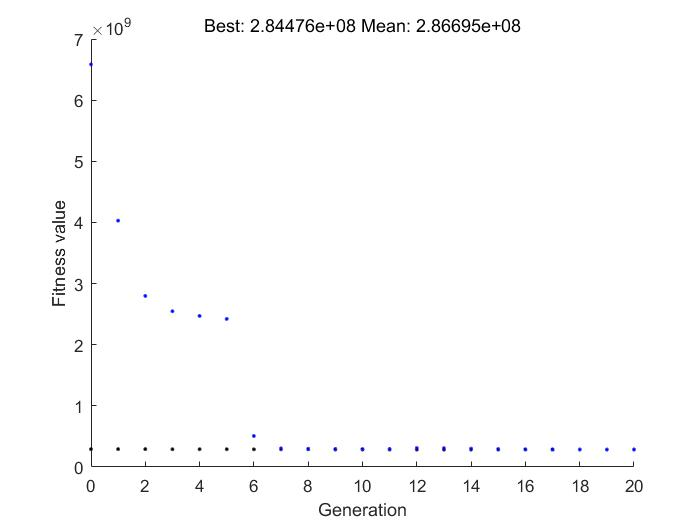
\includegraphics[width = 8cm]{images/GA_jizuiquxian.jpg}
            \caption{GA进化图}
            \label{fig:GA进化图}
            \end{figure}
            \par
            求解得到的最优解$h_1 =17.5mm,h_2=6.4mm$。最优解插值形成的脊椎曲线如图(\ref{三次样条插值求解的人体脊椎曲线})所示
            \begin{figure}[H]
            \centering
            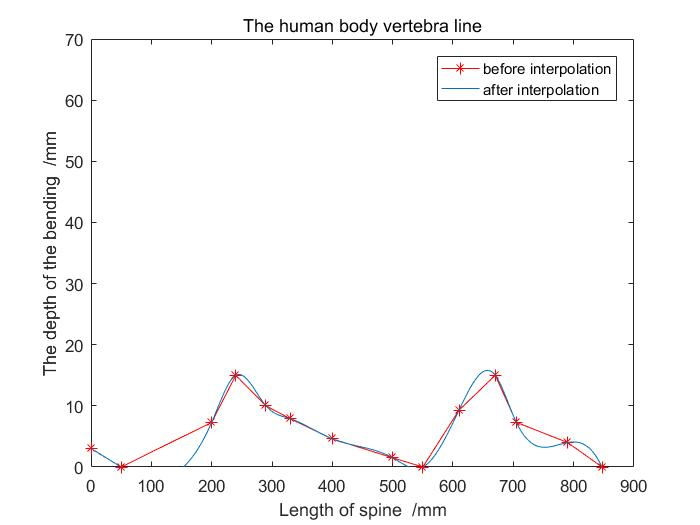
\includegraphics[width = 8cm]{images/jizuiquxian_sanciyangtiao.jpg}
            \caption{三次样条插值求解的人体脊椎曲线}
            \label{三次样条插值求解的人体脊椎曲线}
            \end{figure}
            可以发现,三次样条插值得到的脊椎曲线必过测量点$x_i,y_i$,这使得脊椎曲线并不是很规则,可换用其它插值方法进行求解。
            \par
            \textbf{(3)多项式拟合}
            \par
            每给一个$h_1,h_2$,都会形成一组脊椎测量数据$x_i,y_i$,我们选用某种回归/拟合方法对这组数据进行回归,设回归后的回归函数为$S(x)$。我们求最优的$h_1,h_2$,使得$S(x)$在腰椎和肩胛骨这两个点的曲率分别为1000和500。
            \par
            在求解$h_1,h_2$之前,我们先来确定用什么回归/拟合方法。这里我们选用多项式拟合方法(还可以选取广义线性回归、傅里叶多项式等)。下面我们来确定多项式的最高项阶数,即确定用几次多项式拟合。对人体坐姿数据进行不同的多项式拟合,将多项式拟合的最高次项阶数设置为从1到7,得到各个多项式拟合的拟合优度$R^2$,比较这7个多项式的拟合效果。各个多项式对坐姿数据的拟合效果如图(\ref{7个多项式拟合坐姿数据效果图})所示,各个多项式的$R^2$变化如图(\ref{7个多项式拟合f的R2变化图})所示。
                \begin{figure}[H]
                    \centering
                    \begin{subfigure}[b]{0.4\textwidth}
                        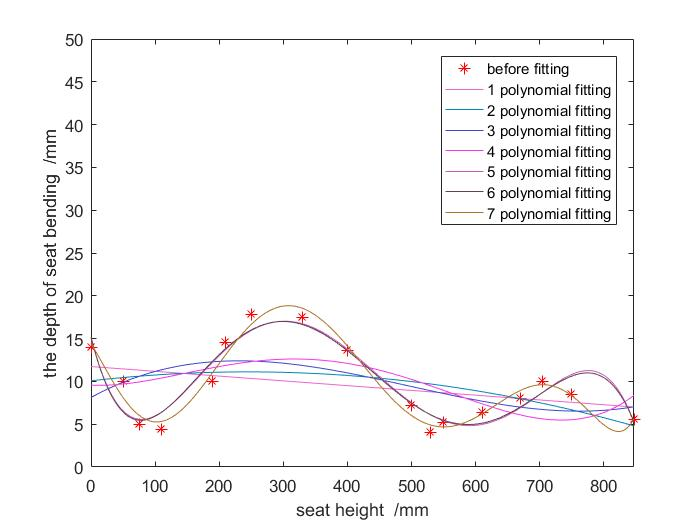
\includegraphics[width=\textwidth]{images/7polynomial_fit_sitting_data.jpg}
                        \caption{7个多项式拟合坐姿数据效果图}
                        \label{7个多项式拟合坐姿数据效果图}
                    \end{subfigure}
                    \begin{subfigure}[b]{0.4\textwidth}
                        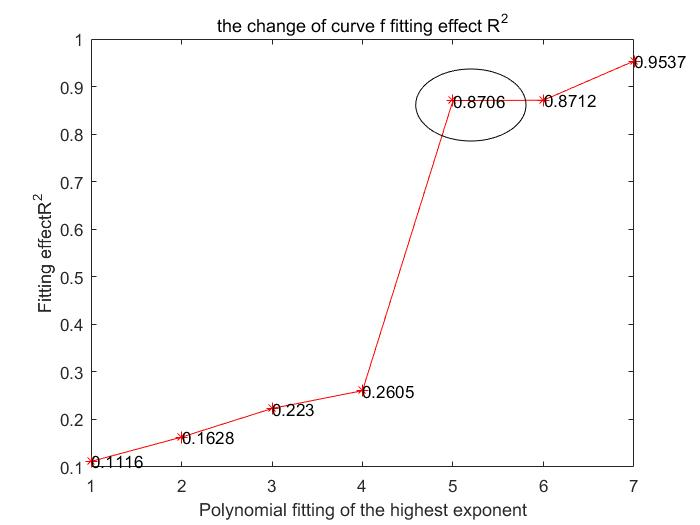
\includegraphics[width=\textwidth]{images/7polynomial_fit_fR2.jpg}
                        \caption{7个多项式拟合f的R2变化图}
                        \label{7个多项式拟合f的R2变化图}
                    \end{subfigure}
                    % \caption{心形图运行结果}
                    % \label{心形图运行结果}
                \end{figure}
            \par
            从图(\ref{7个多项式拟合f的R2变化图})中我们可以看到7次多项式对坐姿数据的拟合效果最好,拟合优度$R^2$为0.9537,5次多项式的拟合优度$R^2$变化最大。这里,我们不可过分要求$R^2$,所以对坐姿数据采用5次多项式拟合
            \begin{align*}
            S(x) = a_0+a_1x+a_2 x^2 + a_3 x^3+a^4x_4+a_5x^5
            \end{align*}
            \par
            仍然选用GA算法来求解最优的$h_1,h_2$,得到的最优深度为$h_1 =17.5mm,h_2=6.4mm$
            最优拟合脊椎曲线为
            \begin{align*}
            f^* = S(x) = 15.08 + 0.002706x^4 - 0.2852x^5
            \end{align*}
            如图(\ref{人体脊椎曲线的5次多项式拟合})所示
            \begin{figure}[H]
            \centering
            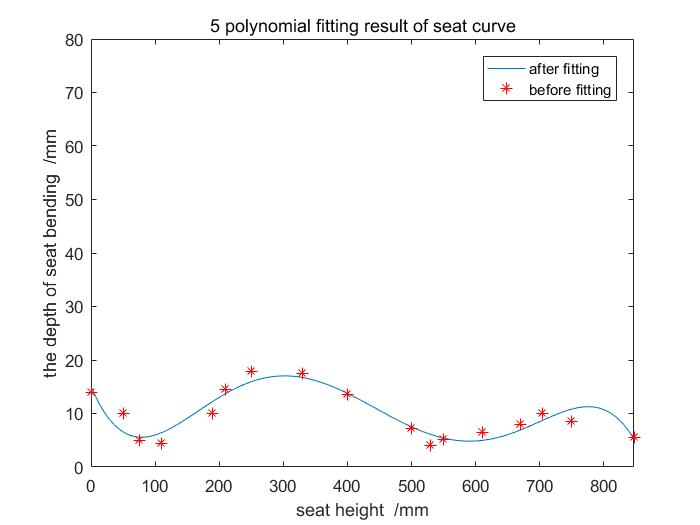
\includegraphics[width = 8cm]{images/jizuiquxian_5ciduoxiangshi.jpg}
            \caption{人体脊椎曲线的5次多项式拟合}
            \label{人体脊椎曲线的5次多项式拟合}
            \end{figure}
            得到的脊椎曲线(座椅曲线)$f$的拟合误差如表(\ref{座椅曲线5次多项式拟合的误差信息表})所示
        \begin{table}[H]
        \centering
        \caption{座椅曲线5次多项式拟合的误差信息表}
        \label{座椅曲线5次多项式拟合的误差信息表}
        \begin{tabular}{cccc}
        \toprule
        多项式系数  & 取值&95\%置信下限 &95\%置信上限\\
        \midrule
        a0 &  -5.232e-12&   -6.831e-12 &  -3.632e-12\\
        a1 &  1.142e-08 &   8.001e-09 &   1.485e-08\\
        a2 &  -8.736e-06 &  -1.135e-05 &  -6.12e-06\\
        a3 &  0.002706 &    0.001854 &    0.003559\\
        a4 &  -0.2852&  -0.3936&  -0.1769\\
        a5 &  15.08  &  11.04 &   19.13\\
        \bottomrule
        \multicolumn{4}{l}{\footnotesize 模型信息为SSE:41.95,R-square:0.8706,AdjustedR-square: 0.8117,RMSE: 1.953}\\
        \end{tabular}
        \end{table}

    \subsection{问题二的分析与求解}
        \subsubsection{问题的分析}
            \par
            问题二要求我们在不改变主内部结构的情况下,优化座椅背板曲线并保证在舒适的前提下使得填充物尽可能的少。首先我们根据问题一的求解可以获得有关机舱座椅设计的空间坐标值,同时我们定义舒服的状态就是主要支撑点的压强$P_i$尽可能的小,在一些条件的约束下设计算法完成压强较小情况的座椅背板最优曲线设计。
        \subsubsection{模型的建立与求解}
            \par
            \textbf{(1)设计超薄飞机座椅的依据}
            \par
            在设计座椅时,有两方面的因素是需要我们着重考虑的,因为我们的座椅是新型超薄型座椅。设计时,考虑的第一个因素是:空间。超薄座椅应该占有更少的空间,也就是说,座椅本身的体积$V$要小,座椅的填充物要少,这样可以给乘客提供更多的活动空间;考虑的第二个因素是:舒适度。超薄座椅应该给旅客提供舒适的旅途服务。想象这样两种情况:\ding{172}当你的后背完全被座椅包裹\ding{173}你的后背停靠在一张木板上。毫无疑问的是第\ding{172}种情况会给人更好的舒适感,这是因为在人体的重量$G$一定的条件下,背部和座椅的接触面积越大,人体给脊椎带来的压强P越小。以坐垫宽为$x$轴,坐垫长度为$y$轴,椅背高为$z$轴建立空间直角坐标系。绘制一张简单的人体脊椎受力图,如图(\ref{人体背部脊椎压力侧视图})所示:设座椅的最优倾斜角度为$\alpha_{best}$ ($0^\circ<\alpha_{best}<30^\circ$ ),人体上半部分的重量为$G⁄2$,对脊椎进行受力分析。
            \begin{figure}[H]
            \centering
            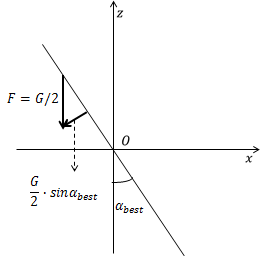
\includegraphics[height = 4.5cm]{images/body_back_spine_pressure_side_view.jpg}
            \caption{人体背部脊椎压力侧视图}
            \label{人体背部脊椎压力侧视图}
            \end{figure}
            \par
            在情况\ding{173}的条件下,是整个脊椎承担$\sin \alpha_{best}G/2$,在情况\ding{172}的条件下,是整个背部承担$\sin \alpha_{best}G/2$,情况\ding{172}给我们提供更多的舒适感。然而,情况\ding{172}需要我们付出更多的座椅填充物,这与我们设计的超薄座椅理念不符。因此,我们有必要研究一下座椅包裹多少使得座椅既舒适又超薄?绘制一个简易的座椅包裹人体的示意图,如图(\ref{座椅包裹人体的俯视图})所示:考虑一个一般的情况,脊椎和座椅的接触点为原点$O$,座椅宽度为$W$,人体躯干宽度为$W_{max}$,人体背部厚度为$d_{max}$,背部曲线为$f$(不妨将其设为二次曲线$y=ax^2$)。
            \begin{figure}[H]
            \centering
            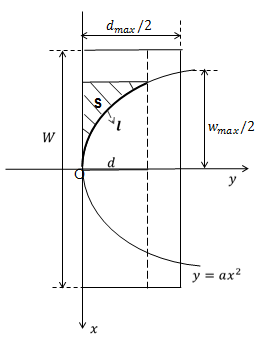
\includegraphics[height = 5cm]{images/seat_covers_the_top_view_human_body.jpg}
            \caption{座椅包裹人体的俯视图}
            \label{座椅包裹人体的俯视图}
            \end{figure}
            \par
            当我们的包裹深度为$d$时,所需要的填充物体积为$2S\Delta H$($\Delta H$为高度微元),背部和座椅的接触面积为$2l\Delta H$($\Delta H$为高度微元)。
            \par
            很显然,我们的目标是求解包裹深度$d$。$d$应该满足单层目标
            \begin{align*}
            & \min\ S=\int_{0}^d (y/a)^{\frac{1}{2}}\mathrm{d}y = \int_{0}^{(d/a)^{1/2}} ax^2 \mathrm{d}x\\
            & \max\ l=\int_{0}^{(d/a)^{1/2}}\sqrt{1+(2ax)^2}\mathrm{d}x\\
            & s.t.\quad 0 \leqslant d \leqslant d_{max}
            \end{align*}
            \par
            上面模型仅考虑了座椅和背部在某一特定的切面上的情况,现在将其推广到空间上。以坐垫宽为$x$轴,坐垫长度为$y$轴,椅背高为$z$轴建立空间直角坐标系,绘制座椅和背部接触包裹的立体图,如图(\ref{座椅和背部接触包裹的立体图})所示:我们设定座椅的高度为$H$,设计的座椅包裹高度为$h$($h$为人体颈椎高度,$h=640mm$),包裹深度$d$离散化为$\{d_i \}_n$($n$为样本点数目),实际上包裹深度曲线$d_f$是光滑的,可以设置整体目标为
            \begin{align}
            \label{飞机超薄座椅模型1}
            & \min \ S=\int_0^h S_i\mathrm{d}z = \sum_{i=1}^n S_i\\
            & \max \ l=\int_0^h l_i\mathrm{d}z = \sum_{i=1}^n l_i\\
            & s.t.\left\{
            \begin{aligned}
            & 0 \leqslant d_i \leqslant d_{i_{max}}\\
            & i=1,2,\dots,n
            \end{aligned}
            \right.\notag
            \end{align}
            \par
            最终,问题转化为求解一组关于$d_i$ 的集合即$\{d_i \}$,$\{d_i \}$使得目标函数(\ref{飞机超薄座椅模型1})同时达到比较好的情况。
            \begin{figure}[H]
            \centering
            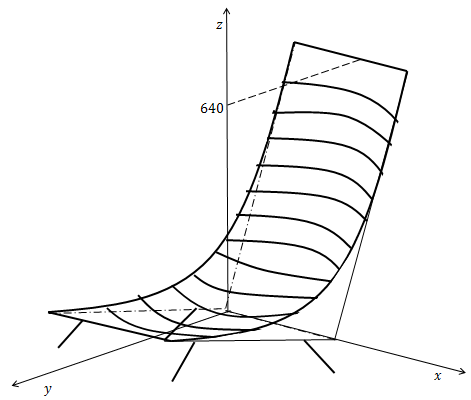
\includegraphics[height=4cm]{images/seat_and_back_near_parcel.jpg}
            \caption{座椅和背部接触包裹的立体图}
            \label{座椅和背部接触包裹的立体图}
            \end{figure}
            \par
            \textbf{(2)超薄座椅包裹深度的优化求解}
            \par
            上述包裹深度的求解问题是一个多目标优化问题。它需要求解一系列的包裹深度$\{d_i \}$或包裹深度曲线$d_f$。在实际问题的应用求解过程中,我们可以根据每家航空公司的偏好设置模型(\ref{飞机超薄座椅模型1})
            目标1和目标2权重,进而求解出优良的$\{d_i \}$。
            \par
            如果希望使顾客有更大的活动空间,需要超薄座椅占据尽可能小的空间,我们可以增加模型(\ref{飞机超薄座椅模型1})目标函数1的权重。如果希望顾客有更舒适的旅途环境,更好的休息条件,我们可以增加目标函数2的权重。同时目标函数1和2的权重之和应该为1。
            \par
            现在,我们给出包裹深度问题的一种求解方法:由于各层的包裹深度曲线$d_f$是光滑的,而且变动幅度很小,这里我们不妨将包裹深度曲线假设为5次多项式函数(当然,我们也可以假设为傅里叶多项式,这里不做介绍):
            \begin{align*}
            d_f = a_0+a_1z+a_2z^2+a_3z^3+a_4z^4+a_5z^5
            \end{align*}
            \begin{figure}[H]
            \centering
            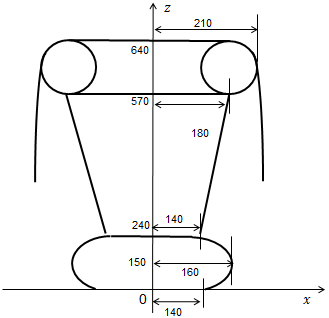
\includegraphics[height=4.5cm]{images/body_back_special_segment.jpg}
            \caption{人体背部特殊部位}
            \label{人体背部特殊部位}
            \end{figure}
            \par
            然后选取人体背部$n$个特殊部分如图(\ref{人体背部特殊部位})所示,求解其对应的$\{d_i \}_n$,并对$\{d_i \}_n$利用多项式拟合,也可以进行三次样条插值或者B样条插值,使得$\{d_i \}$更加光滑。选取的人体背部$n$个特殊部位的数据如表(\ref{人体背部n个特殊部位宽度和厚度数据})所示
        \begin{table}[H]
        \centering
        \caption{人体背部n个特殊部位宽度和厚度数据}
        \label{人体背部n个特殊部位宽度和厚度数据}
        \begin{tabular}{cccccc}
        \toprule
        {}&   坐板 & 臀部 & 腰部 & 胸部 & 肩部\\
        \midrule
        $z$ &  0   & 150 & 240& 570 & 640\\
        $x$ &  140 & 160 & 140& 180 & 210\\
        $y$ &  30  & 65  & 30 & 76  & 70\\
        \bottomrule
        \multicolumn{6}{l}{\footnotesize 注:$x$为$1/2$的$w_max$;$y$为$1/2$的$d_max$。}\\
        \end{tabular}
        \end{table}
            % \textcolor[rgb]{1 0 0}{todo:表格:人体背部n个特殊部位宽度和厚度数据}\\
            \par
            对如表(\ref{人体背部n个特殊部位宽度和厚度数据})中的数据进行等间距采样后的$n$个特殊部位的数据如表(\ref{等间距采样后的n个特殊部位宽度和厚度数据})所示,这里假设人体背部侧轮廓曲线为直线。
        \begin{table}[H]
        \centering
        \caption{等间距采样后的n个特殊部位宽度和厚度数据}
        \label{等间距采样后的n个特殊部位宽度和厚度数据}
        \begin{tabular}{cccccccc}
        \toprule
        % {}&   坐板 & 臀部 & 腰部 & 胸部 & 肩部\\
        % \midrule
        $z$ & 1.00   & 50.00  & 100.00 & 150.00 & 200.00 & 240.00 & 300.00\\
        $x$背宽 & 140.00 & 146.58 & 153.29 & 160.00 & 148.99 & 140.00 & 147.17\\
        $y$体厚  & 30.00  & 41.51  & 53.26  & 65.00  & 45.73  & 30.00  & 38.25 \\
        \hline
        \hline
        $z$ & 350.00 & 400.00 & 450.00 & 500.00 & 570.00 & 600.00 & 640.00\\
        $x$背宽 & 153.25 & 159.33 & 165.41 & 171.49 & 180.00 & 192.61 & 210.00\\
        $y$体厚 & 45.24  & 52.23  & 59.22  & 66.21  & 76.00  & 73.48  & 70.00 \\
        \bottomrule
        \multicolumn{8}{l}{\footnotesize 注:$z$为座椅高度;$d$为最优包裹深度。}\\
        \end{tabular}
        \end{table}

            \par
            在采集样本的过程中,假设人体背部的侧轮廓线为一次曲线,我们可以通过采样获取更多的样本点,这对插值和曲线拟合均有很大帮助。
            \par
            运用IENSGA\rom{2}求解$\{d_i \}_n$,IENSGA\rom{2}的参数设置为: 'ParetoFraction':0.3,'PopulationSize':100,' Generation':200,'StallGenLimit':200,'TolFun':1e-100,设置变量的取值范围:$0 \leqslant d \leqslant d_{i_{max}}$。利用表(\ref{人体背部n个特殊部位宽度和厚度数据})的数据得到的pareto最优进化图如图(\ref{表4下pareto最优进化图})所示;在表(\ref{等间距采样后的n个特殊部位宽度和厚度数据})等间距采样后的数据下求得的pareto最优进化图为图(\ref{表5下pareto最优进化图})
                \begin{figure}[H]
                    \centering
                    \begin{subfigure}[b]{0.4\textwidth}
                        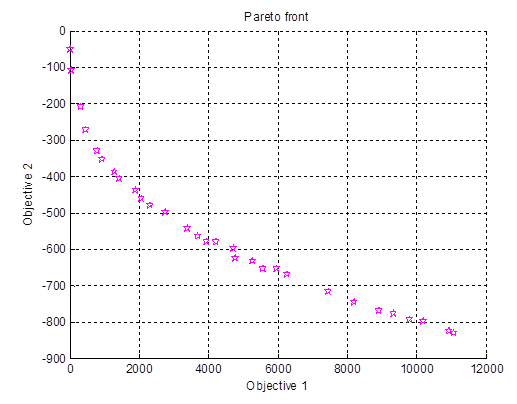
\includegraphics[width=\textwidth]{images/tab4_pareto.png}
            \caption{表(\ref{人体背部n个特殊部位宽度和厚度数据})下pareto最优进化图}
            \label{表4下pareto最优进化图}
                    \end{subfigure}
                    \begin{subfigure}[b]{0.4\textwidth}
                        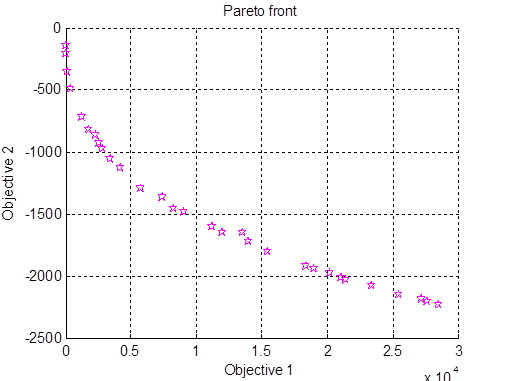
\includegraphics[width=\textwidth]{images/tab5_pareto.png}
            \caption{表(\ref{等间距采样后的n个特殊部位宽度和厚度数据})下pareto最优进化图}
            \label{表5下pareto最优进化图}
                    \end{subfigure}
                    % \caption{心形图运行结果}
                    % \label{心形图运行结果}
                \end{figure}

            \par
            在Pareto最优解中选择一个适当的个体(解),在选择时,考虑到我们是设计超薄座椅,当我们选择利用目标函数1获取较小解时,选取图(\ref{表5下pareto最优进化图})中10个解如表(\ref{IENSGA2某次求解的结果的10个解})所示,解对应的目标函数1取值结果为:4225(体积)。相应的若选取目标函数2获取较小解时,目标函数2取值结果:-1229(舒适度)。

        \begin{table}[H]
        \centering
        \caption{IENSGA2某次求解的结果的10个解}
        \label{IENSGA2某次求解的结果的10个解}
        \begin{tabular}{cccccccc}
        \toprule
        % {}&   坐板 & 臀部 & 腰部 & 胸部 & 肩部\\
        % \midrule
        $z$  & 1.00   & 50.00 &  100.00 & 150.00 & 200.00 & 240.00 & 300.00\\
        $d$  & 8.51   & 11.38 &  19.42  & 30.84  & 6.03   & 12.44  & 12.67 \\
        \hline
        \hline
        $z$  & 350.00 & 400.00&  450.00 & 500.00 & 570.00 & 600.00 & 640.00\\
        $d$  & 13.88  & 8.51  &  14.89  & 20.36  & 13.30  & 3.62   & 12.38 \\
        \bottomrule
        \multicolumn{8}{l}{\footnotesize 注:$z$为座椅高度;$d$为最优包裹深度。}\\
        \end{tabular}
        \end{table}
            \par
            在上述的过程中,我们通过提取人体背部的一些特殊部分求解了相对应的最优包裹深度$\{d_i \}_n$,然后,我们对样本点进行插值和5次多项式拟合使包裹曲线更加光滑,得到的5次多项式为
            \begin{align*}
            d_f = 5.481-0.0348z^4+0.3939z^5
            \end{align*}
            拟合结果如图(\ref{最佳包裹深度的插值和5次多项式拟合结果})所示
            \begin{figure}[H]
            \centering
            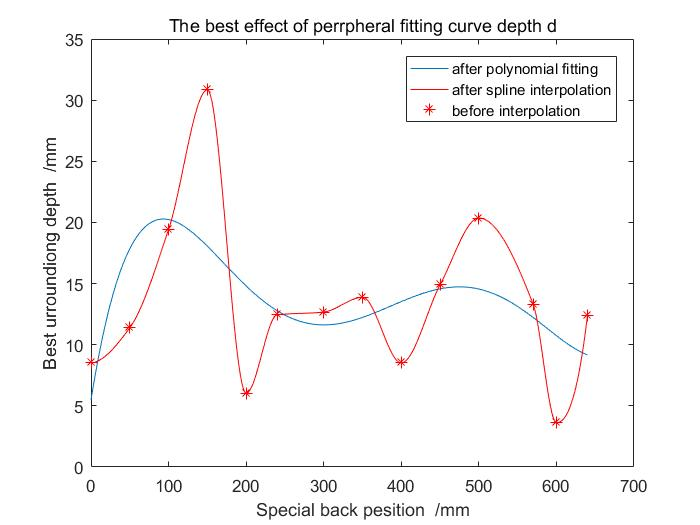
\includegraphics[width=8cm]{images/optimal_parcel_depth_interpolation_and_5polynomail.jpg}
            \caption{最佳包裹深度的插值和5次多项式拟合结果}
            \label{最佳包裹深度的插值和5次多项式拟合结果}
            \end{figure}
            \par
            \textbf{(3)超薄座椅的3D设计方案}
            \par
            在进行座椅的3D设计时,我们需要根据乘客的坐姿(脊椎)数据、座椅的最优曲线$f$、座椅包裹背部的最优深度$d_f$为参考进行设计。设计3D座椅时,考虑到乘客的头部需要很大的活动空间,不可以将其过分固定,所以我们不对头部进行包裹,因此,设计的座椅的做大背部包裹为640mm。下面给出座椅贴近背部的曲面3D示意图,如图(\ref{座椅与人体背部贴近曲面的3D示意图})所示
                \begin{figure}[H]
                    \centering
                    \begin{subfigure}[b]{0.4\textwidth}
                        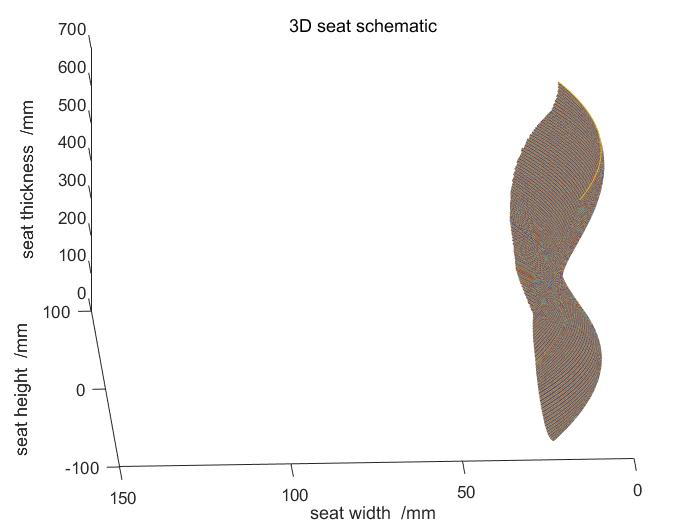
\includegraphics[width=\textwidth]{images/seat_body_back_near_curve1.jpg}
                        % \caption{}
                    \end{subfigure}
                    \begin{subfigure}[b]{0.4\textwidth}
                        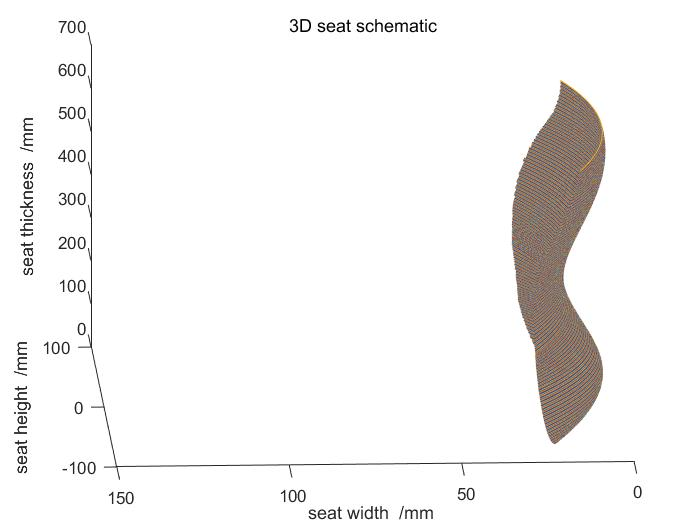
\includegraphics[width=\textwidth]{images/seat_body_back_near_curve2.jpg}
                        % \caption{}
                    \end{subfigure}
                    \begin{subfigure}[b]{0.4\textwidth}
                        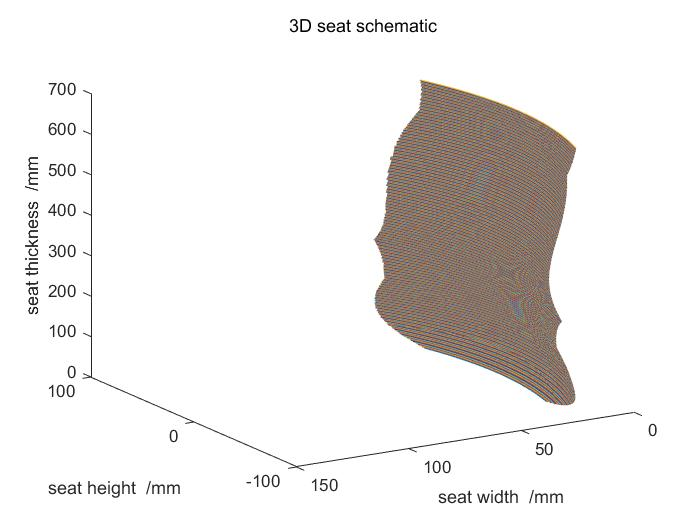
\includegraphics[width=\textwidth]{images/seat_body_back_near_curve3.jpg}
                        % \caption{}
                    \end{subfigure}
                    \begin{subfigure}[b]{0.4\textwidth}
                        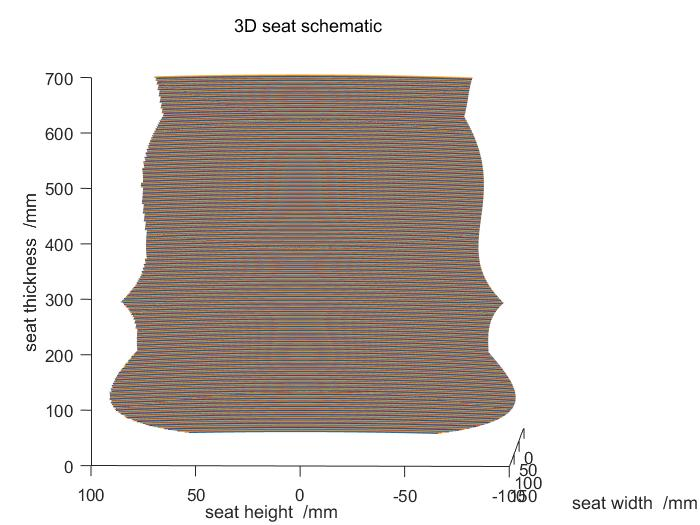
\includegraphics[width=\textwidth]{images/seat_body_back_near_curve4.jpg}
                        % \caption{}
                    \end{subfigure}
                    \caption{座椅与人体背部贴近曲面的3D示意图}
                    \label{座椅与人体背部贴近曲面的3D示意图}
                \end{figure}

            \par
            在我们设计座椅包裹背部的3D曲面时,我们对座椅曲线$f$进行3次样条插值,并结合了5次多项式拟合的结果,选取背部特殊部位,计算包裹深度,选取比较恰当的pareto解(第10个解),然后对包裹深度$d$进行5次多项式拟合。
        \subsubsection{pareto解的选取/目标偏好对包裹深度$d_f$的敏感性分析}
            \par
            3在求解座椅和背部的包裹曲线$d_f$的时候,我们在人体背部选取了$n$个特殊部位,然后再得到的pareto最优解中依据目标偏好选取了某一个解$\{d_i \}_n$对其进行拟合,现在,我们有必要研究不同的pareto最优解$\{d_i\}_n$的5次多项式拟合$d_f$的效果,以及特殊点的数目$n$(样本量)对拟合$d_f$的影响。
            \par
            选取某一次求解的pareto最优解中的所有的解,对它们进行5次多项式拟合,拟合效果如图(\ref{Pareto最优解的5次多项式拟合})所示,从图中我们可以看出:如果我们希望给旅客提供尽可能大的活动空间(目标1的偏好严重),座椅对人体背部的包裹深度$d_f$几乎处处为0(如图(\ref{Pareto最优解的5次多项式拟合})最下面的曲线);如果我们希望给旅客提供最舒服的旅程(目标2的偏好严重),座椅会对人体提供最大的包裹深度$d_f$(如图(\ref{Pareto最优解的5次多项式拟合})最上面的曲线)。从整体来看,$\{d_f \}$在人体背部的尾部变化较小,肩部变化较大,这是因为肩部有更大的体积变化幅度。
            \begin{figure}[H]
            \centering
            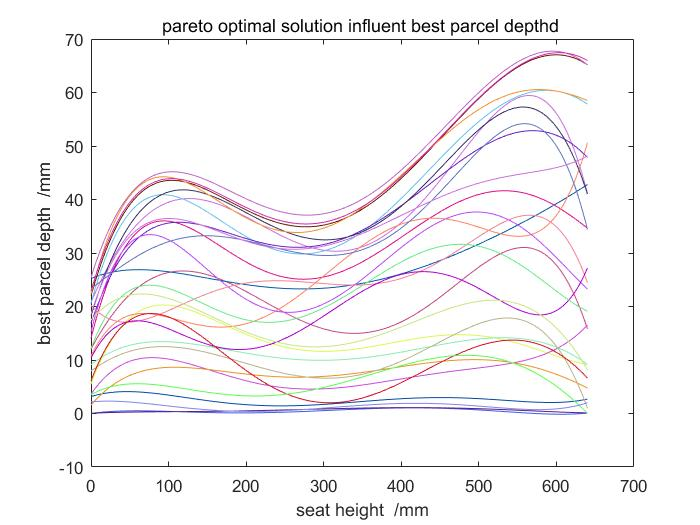
\includegraphics[width=8cm]{images/effect_pareto_df.jpg}
            \caption{Pareto最优解的5次多项式拟合$\{d_f \}$($n=15$)}
            \label{Pareto最优解的5次多项式拟合}
            \end{figure}
            \par
            接下来,我们研究特殊点的数目$n$(样本量)对拟合$d_f$的影响。选取人体背部的5和15个特殊部位($n=5\&15$),分别研究他们的pareto最优解的5次多项式拟合,$n=5$时的拟合结果如图(\ref{Pareto最优解的5次多项式拟合n为5时})所示,$n=15$的拟合结果如图(\ref{Pareto最优解的5次多项式拟合})所示。比较这两幅图的差别,我们可以看到:$n=5$样本点少的时候,pareto最优解的5次多项式拟合$\{d_f \}$的变动幅度更大,也就是说,当我们的$n$足够大时,$\{d_f \}$将接近真实的$d_f^{best}$。
            \begin{figure}[H]
            \centering
            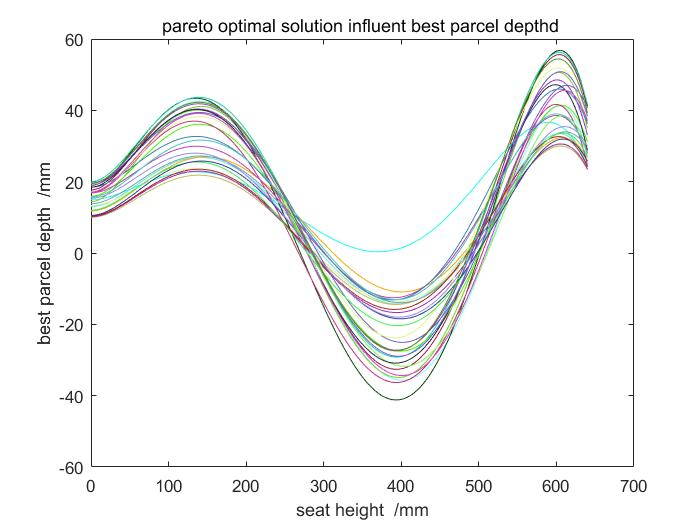
\includegraphics[width=8cm]{images/effect_pareto_df_2.jpg}
            \caption{Pareto最优解的5次多项式拟合$\{d_f \}$($n=5$)}
            \label{Pareto最优解的5次多项式拟合n为5时}
            \end{figure}

        \subsubsection{程序}
            \par
            IENSGA\rom{2}的目标函数如下
            \begin{lstlisting}[language = Matlab]
            function Obj = obj2fun_15(d)
            % 求解背部二次曲线
            % 前提假设:1.背部曲线为二次曲线;
            %           2.背部的侧轮廓为一次直线;
            % 参数:宽度(w)xi,厚度(thick)yi
            index = [0 150 240 570 640];                     %z特殊位置
            x = [140 160 140 180 210];                       %1/2的宽度
            y = [30 65 30 76 70];                            %1/2的厚度
            % 依据标度index对xy进行扩充
            nnn = length(index);
            for i = 1:nnn-1
                newx = [newx,linspace(x(i),x(i+1),index(i+1)-index(i))];
                newy = [newy,linspace(y(i),y(i+1),index(i+1)-index(i))];
            end
            % 计算二次曲线参数a=y/x^2
            a = newy./(newx.^2);
            ind_z=[1 50 100 150 200 240 300 350 400 450 500 570 600 640];
            n = length(ind_z);
            % 求面积S和弧长L(有对称性可知,只需求解在第一挂限的情况即可*2)
            aa = a(ind_z);
            x = (d./aa).^(1/2);%d=ax^2
            for i=1:n
                S(i, 1) = integral(@(xx)a(i)*xx.^2,0,x(i));% 求fi的面积0-xi(积分)
                L(i, 1) = integral(@(xx)(1+(2*a(i)*xx).^2).^(1/2),0,x(i));%求fi的弧长
            end
            Obj(1) = sum(S);
            Obj(2) = -sum(L);
            \end{lstlisting}
            IENSGA\rom{2}的主程序如下
            \begin{lstlisting}[language = Matlab]
            %% 多目标优化IENSGA2的主程序
            % min min 类型的多目标优化
            clc,clear
            fitnessfun = @obj2fun_15;%适应度函数句柄
            % 确定变量个数di
            ind_z=[1 50 100 150 200 240 300 350 400 450 500 570 600 640];
            nvars = length(ind_z);%变量个数
            % 确定变量取值范围lb,ub
            index = [0 150 240 570 640];                   %z特殊位置
            x = [140 160 140 180 210];                     %1/2的宽度
            y = [30 65 30 76 70];                          %1/2的厚度
            % 依据标度index对xy进行扩充
            nnn = length(index);
            for i = 1:nnn-1
                newx = [newx,linspace(x(i),x(i+1),index(i+1)-index(i))];
                newy = [newy,linspace(y(i),y(i+1),index(i+1)-index(i))];
            end
            %%%%%%%%%%%%GA自变量di的范围%%%%%%%%%%%
                              %第一种情况:在最大值的1/3,2/3范围
                                        % lb=newy(ind_z)/3;
                                        % ub=2*newy(ind_z)/3;
                              %第二种情况:在0:最大值范围
                                          lb=zeros(1,nvars);
                                          ub=newy(ind_z);
            %%%%%%%%%%%%非常关键的地方%%%%%%%%%%%%%
            A=[];b=[];Aeq=[];beq=[];
            options=gaoptimset('ParetoFraction',0.3,...
                               'PopulationSize',100,...
                               'Generation',200,...
                               'StallGenLimit',200,...
                               'TolFun',1e-100,...
                               'PlotFcns',@gaplotpareto);
            [d_index,Obj]=gamultiobj(fitnessfun,nvars,A,b,Aeq,beq,lb,ub,options);
            \end{lstlisting}




% \bibliography{}%bib文件名称
% \end{document}
